\documentclass{article}
\usepackage[utf8]{inputenc}

\title{Tarea 2: Frogger}
\author{Andrés José Ramirez Ortega}
\date{April 2021}

\usepackage{natbib}
\usepackage{graphicx}


\begin{document}

\maketitle

\section{Introducción}
Frogger es un juego de arcade desarrollado por Konami y originalmente publicado por Sega. El objetivo del juego es guiar a las ranas a sus hogares, una por una, cruzando carreteras y rios con muchos peligros. Este juego ha encontrado su lugar en la cultura popular, incluyendo la televisión y la música. El objetivo del programa realizado es desarrollar una aplicación utilizando el lenguaje de programación Ensamblador, que permita comprender el arranque de un Sistema Operativo.

\begin{figure}[h!]
\centering
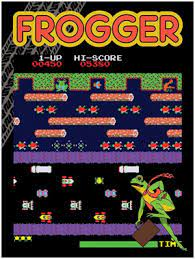
\includegraphics[scale=0.5]{frogeers.jpg}
\caption{Imagen del juego Frogger.}
\label{fig:frogeers}
\end{figure}

En nuestro programa, el juego Frogger consiste en una rana que trata de pasar por almenos 3 calles, en las cuales transitan diferentes tipos de carros. Los automoviles tienen un largo de 1, las busetas tienen un largo de 2 y los camiones corrsponden a largo 3. Si se logra pasar por todos los carriles sin que sea colisionado, el jugador gana. 

\subsection{Requerimientos}
\begin{itemize}
    \item Se debe utilizar el lenguaje de programación Ensamblador para x86.
    \item EFI será el mecanismo de booteo.
    \item Programar en ensamblador el booteo desde una unidad de USB.
    \item Una vez que bootee desde el USB, cargará única y exclusivamente un programa llamado: Frogger. 
\end{itemize}
\section{Ambiente de desarrollo}

Las herramientas utilizadas para la elaboración y la implemnetación de la tarea corta 2 fueron las siguientes: 

\begin{itemize}
    \item Se utilizó una laptop HP, con 12 GB de RAM y un sistema x64. 
    \item Un Sistema Operativo Ubuntu 20.04, el cual fue trabajado sobre una Oracle VirtualBox. 
    \item Las pruebas fueron realizadas sobre la VirtualBox. 
    \item El compilador del código ensamblador x86 fue Fasm, aunque también se realizaron pruebas en Masm y Nasm. 
    \item Se utiliza la biblioteca uefi.inc para importar los diferentes headers necesarios en el código. 
\end{itemize}

\section{Estructuras de datos usadas y Funciones}
\subsection{Estructuras}
La estructura utilizada es una matriz, en la cual existen 5 carriles por donde pasan los carros. Los carros pasan por los carriles del medio y las filas 1 y 5 son los carriles seguros. Si el jugador llega a la fila 1 significa que ya ganó. 
\subsection{Funciones}
Entre las funciones más importantes se encuentran:
\begin{itemize}
    \item Mover el frog: Estas funciones toman la entrada del usuario y realizan el movimiento del frog en el tablero dependiendo de la entrada. 
    \item Mover los vehiculos: Esta función realiza el movimiento de los vehículos sobre los carriles del juego, además implementa funciones de validación para no salirse del tamaño de la matriz. 
    \item Funciones de validación: Validan el movimiento de todos los agentes presentes en el juego, asegurandose de que no se salgan del tablero si llegan a un punto donde ya no se puede mover. También ayudan a agilizar el movimiento de los vehículos y el frog. 
    \item Funciones de finalización: Estas funciones validan si el frog se encuentra en la primera posición de la matriz, lo cual lo convierte en un ganador, o por el contrario choca con algún vehículo y pierde. 
    \item Funciones de la biblioteca uefi.inc, las cuales nos permiten realizar operaciones sobre pantalla, imprimir datos, limpiar la pantalla y obtener los datos desde el teclado. 
\end{itemize}
\section{Instrucciones para ejecutar el programa}
Los pasos son los siguientes: 
\begin{enumerate}
    \item Primeramente se debe instalar Fasm mediante el comando - sudo apt-get install -y fasm.
    \item Luego creamos una carpeta donde se va a encontrar el proyecto. La carpeta puede tener cualquier nombre. 
    \item Dentro de esta carpeta se crearán dos carpetas más. Una carpeta llamada efi y dentro de esta carpeta se creará otra llamada boot. 
    \item Ya con las carpetas creadas, abrimos una terminal en la cual vamos a correr el siguiente comando - fasm frogger.asm. 
    \item Al ejecutar el comando, se creará un archivo frogger.efi, este archivo debe estar dentro de la carpeta boot y se le debe cambiar el nombre a "bootx64.efi". 
    \item Ya con el archivo "bootx64.efi" dentro de boot, ejecutamos el siguiente comando - mkisofs -o frogger.iso ./carpeta, donde carpeta es el nombre de la carpeta que creamos al inicio. 
    \item Este comando nos creará el Frogger.iso, que lo utilizaremos proximamente en la máquina virtual. 
    \item Creamos una nueva máquina virtual con las opciones por defecto, en las cual iremos a su configuración y en el apartado de sistema habilitaremos el Efi. Además de esto, debemos agregar el Frogger.iso en la parte de almacenamiento. 
    \item Por último, inicializamos la máquina virtual y jugamos. 
\end{enumerate}

\section{Autoevaluación}
El estado final del Frogger es que cumple con la mayoría de los requerimientos solicitados, aunque al principio se tuvieron algunos problemas para correr el código ya que presentaba
algunos errores que no entendía. Además, trabajar sobre la máquina virtual hace que el trabajo se vuelva más lento, ya que no tiene tantos recursos y se vuelve lenta e incluso en algunos
momentos se quedaba pegada. 
La calificación incluida con la rúbrica de "Evaluación" es:
\begin{itemize}
    \item Sector de Arranque: 30
    \item Frogger: 45
    \item Documentación: 17 
\end{itemize}
El link del repositorio es https://github.com/andres0599/Tarea2-Frogger.git.

\section{Actividades realizadas por el estudiante}

\begin{tabular}{ |p{3cm}||p{3cm}|p{3cm}|  }
 \hline
 \multicolumn{3}{|c|}{Lista de Actividades} \\
 \hline
 Actividad        & Día   &Cantidad Horas\\
 \hline
 Investigar sobre ensamblador   &22/3/2020     &3 hrs\\
 Instalar la máquina virtual   &23/3/2020     &2 hrs\\
 Instalar los diferentes ambientes de trabajo   &24/3/2020     &3 hrs\\
 Códificar y probar ambiente   &24/3/2020     &2 hrs\\
 Investigar sobre booteo con EFI   &26/3/2020     &4 hrs\\
 Programar funciones básicas del Frogger   &28/3/2020     &4 hrs\\
 Programar movilidad de los autos   &1/4/2020     &2 hrs\\
 Programar movilidad del Frog   &3/4/2020     &4 hrs\\
 Empezar documentación   &4/4/2020     &2 hrs\\
 Documentar el código   &4/4/2020     &4 hrs\\
 Armar el loop del juego   &5/4/2020     &3 hrs\\
 Realizar el booteo   &6/4/2020     &7 hrs\\
 Realizar pruebas   &6/4/2020     &4 hrs\\
 Terminar documentación   &29/3/2020     &3 hrs\\
 \hline
\end{tabular}

\section{Lecciones Aprendidas}
La mayor lección que aprendí fue dedicar la mayor parte de tiempo a investigar sobre codificar, ya que es mucho más fácil codificar algo que usted entiende. En lenguajes como 
ensamblador o rust no hay mucha documnetación o videos que ayuden a entender las cosas, así que si no encuentra información hay que seguir buscando y tratar de entender y 
analizar todo para poder cumplir los objetivos. Ensamblador es un lenguaje difícil, pero también es muy repetitivo, por lo cual el código de las funciones se repite mucho y 
con la práctica se logra entender y mejorar rápidamente. El booteo fue los que menos me costó, ya que tomo menos tiempo, pero no es recomendable dejar todo para el final. Distribuir las horas 
de trabajo y distribuir bien las actividades por realizar es de suma importancia para lograr todos los objetivos y no tener un desgaste mental y físico muy severo. 


\begin{thebibliography}{0}
  \bibitem{Docu} Kevin Moraga.(2021).Documentación Tarea 2
  \bibitem{wiki} Wikipedia contributors. (2021, 27 marzo). Frogger. Wikipedia. https://en.wikipedia.org/wiki/Frogger 
  \bibitem{efi} EFIBootLoaders - Ubuntu Wiki. (s. f.). Ubuntu Wiki. https://wiki.ubuntu.com/EFIBootLoaders
  \bibitem{asemblyguide} Guide to x86 Assembly. (s. f.). Guide. https://www.cs.virginia.edu/%7Eevans/cs216/guides/x86.html
  \bibitem{uefi} Uefi. (s. f.). Wiki. https://wiki.osdev.org/Uefi.inc
  
\end{thebibliography}


\end{document}
